\documentclass{article}\usepackage[]{graphicx}\usepackage[]{xcolor}
% maxwidth is the original width if it is less than linewidth
% otherwise use linewidth (to make sure the graphics do not exceed the margin)
\makeatletter
\def\maxwidth{ %
  \ifdim\Gin@nat@width>\linewidth
    \linewidth
  \else
    \Gin@nat@width
  \fi
}
\makeatother

\definecolor{fgcolor}{rgb}{0.345, 0.345, 0.345}
\newcommand{\hlnum}[1]{\textcolor[rgb]{0.686,0.059,0.569}{#1}}%
\newcommand{\hlsng}[1]{\textcolor[rgb]{0.192,0.494,0.8}{#1}}%
\newcommand{\hlcom}[1]{\textcolor[rgb]{0.678,0.584,0.686}{\textit{#1}}}%
\newcommand{\hlopt}[1]{\textcolor[rgb]{0,0,0}{#1}}%
\newcommand{\hldef}[1]{\textcolor[rgb]{0.345,0.345,0.345}{#1}}%
\newcommand{\hlkwa}[1]{\textcolor[rgb]{0.161,0.373,0.58}{\textbf{#1}}}%
\newcommand{\hlkwb}[1]{\textcolor[rgb]{0.69,0.353,0.396}{#1}}%
\newcommand{\hlkwc}[1]{\textcolor[rgb]{0.333,0.667,0.333}{#1}}%
\newcommand{\hlkwd}[1]{\textcolor[rgb]{0.737,0.353,0.396}{\textbf{#1}}}%
\let\hlipl\hlkwb

\usepackage{framed}
\makeatletter
\newenvironment{kframe}{%
 \def\at@end@of@kframe{}%
 \ifinner\ifhmode%
  \def\at@end@of@kframe{\end{minipage}}%
  \begin{minipage}{\columnwidth}%
 \fi\fi%
 \def\FrameCommand##1{\hskip\@totalleftmargin \hskip-\fboxsep
 \colorbox{shadecolor}{##1}\hskip-\fboxsep
     % There is no \\@totalrightmargin, so:
     \hskip-\linewidth \hskip-\@totalleftmargin \hskip\columnwidth}%
 \MakeFramed {\advance\hsize-\width
   \@totalleftmargin\z@ \linewidth\hsize
   \@setminipage}}%
 {\par\unskip\endMakeFramed%
 \at@end@of@kframe}
\makeatother

\definecolor{shadecolor}{rgb}{.97, .97, .97}
\definecolor{messagecolor}{rgb}{0, 0, 0}
\definecolor{warningcolor}{rgb}{1, 0, 1}
\definecolor{errorcolor}{rgb}{1, 0, 0}
\newenvironment{knitrout}{}{} % an empty environment to be redefined in TeX

\usepackage{alltt}
\usepackage{hyperref}
\usepackage[margin=0.8in]{geometry}
\usepackage{booktabs}
\usepackage{amsmath}
\usepackage{gensymb}
\usepackage{natbib}
\IfFileExists{upquote.sty}{\usepackage{upquote}}{}
\begin{document}
% \SweaveOpts{concordance=TRUE}

\title{Coringtreespotters ms outline}
\author{Christophe Rouleau-Desrochers}
\date{\today}
\maketitle

% Set CoringTreespotters species shortcut
\newcommand{\Arub}{\textit{A. rubrum}}
\newcommand{\Asac}{\textit{A. saccharum}}
\newcommand{\Afla}{\textit{A. flava}}
\newcommand{\Ball}{\textit{B. alleghaniensis}}
\newcommand{\Bnig}{\textit{B. nigra}}
\newcommand{\Cgla}{\textit{C. glabra}}
\newcommand{\Cova}{\textit{C. ovata}}
\newcommand{\Pdel}{\textit{P. deltoides}}
\newcommand{\Qalb}{\textit{Q. alba}}
\newcommand{\Qrub}{\textit{Q. rubra}}
\newcommand{\Tame}{\textit{T. americana}}   




% <><><><><><><><><><><><><><><><><><><><><><><><><><><><><><><><><><><><><><><>
\section*{Introduction}
% <><><><><><><><><><><><><><><><><><><><><><><><><><><><><><><><><><><><><><><>
Anthropogenic climate change affects many different biological processes with one of the most documented being shifts in phenology---the study of recurring life history events \cite{cleland_shifting_2007,menzel_european_2006,parmesan_poleward_1999}. In plants, shifts in spring and autumn phenology have lengthen the window of opportunity during which they can grow \citep{duputie_phenological_2015}. Trees more specifically should grow more with longer growing seasons which is particularly significant given the critical role that forests play in offsetting human-emitted greenhouse gas emissions \citep{keenan_net_2014, stridbeck_partly_2022,harrisGlobalMapsTwentyfirst2021}. In temperate ecosystems, a large portion of that carbon is stored in mature, canopy trees which emphasizes their decisive role in the potential of forest carbon sink [*REF]. \\

However, the long standing assumption that longer growing seasons should increased growth has recently been challenged by studies that failed to find this relationship \citep{dow_warm_2022,silvestro_longer_2023,wang_seasonal_2025,charletdesauvage_temperature_2022,cabon_crossbiome_2022}. Indeed, warmer springs---which contribute in large part to extending the growing season---have not increased maximum tree growth rate or annual increment in a temperate mixed forest community \citep{dow_warm_2022}. Increased tree growth with longer growing season is an important foundation of current carbon models which are crucial tools to guide greenhouse gas emission objectives and their related solutions \citep{friedlingstein_global_2026}. This brings to light the need to understand why trees may not grow more with longer growing seasons. \\ 

Wood anatomy and tree growth strategies may guide tree species responses to growing seasons. Wood anatomy in angiosperm trees impacts their growth temporality where ring-porous species start growing several days or weeks earlier than diffuse-porous species [Savage2022,Hessl2026, dorangeville2021Peak]. As a result, species with different wood anatomy experience considerably different temperature regime during the growing season leading to asymmetric effect of season length on growth across different species. Furthermore, longer growing seasons may benefit slower growth species because appropriate conditions would allow them to keep their low growth rate active for a longer period [*Cuny2012Life]. In contrast, fast-growth species can complete their season growth increment in a short period, making extra days less crucial for them  [*REF]. Additionally, how trees store the carbon that they accumulate (whether it is through a direct investment in growth or for long-term storage) could mute short term responses. These different carbon allocation strategies highlight the importance of considering the GS conditions of more than one year. \\

The previous year thermal conditions can affect the following year's growth. Deciduous trees often use stored carbon at the beginning of the growing season because they need to grow new leaves before starting photosynthesis [*Wolkovich2025, Monson2018Finding]. Mature trees in particular can rely on stored carbon for their early season growth that was stored several years before [*Hessl2026]. This shows that while the environmental conditions during the current year can have a direct effect on growth, it is likely that this poorly understood carbon allocation strategy to storage may be blurred by a multi-year lag effect. \\

Here, we will look at the growth and growing season length relationship of mature trees in an urban arboretum. For this, we used 11 species of mature trees across nine years and looked at the growing season length and thermal conditions during that period. We also investigated the effect of the previous year thermal conditions on the current year growth. We used growth with tree rings and leaf phenology for the start and end of season that citizen scientists collected.

% <><><><><><><><><><><><><><><><><><><><><><><><><><><><><><><><><><><><><><><>
% DISCUSSION
% <><><><><><><><><><><><><><><><><><><><><><><><><><><><><><><><><><><><><><><>
\clearpage
\section*{Discussion}
In this study, we used 49 trees of 11 species to understand if mature trees grew more with longer growing seasons (GS). To do this, we used annual growth with tree rings and leaf phenology for the SOS and EOS. Our findings reveal that warmer and longer GS did not increase growth for any species and decreased growth for one. We also found that the previous year thermal conditions shifted growth trends for two species. Finally, most species did not respond to the start and end of the GS. \\

While our species share an array of growth strategies, we did not find a consistent growth trend across them. The thermal and calendar season had no effect on any species, except for one. {\Ball} growth decrease with warmer thermal seasons suggests that this species growth may be inhibited by warmer seasons. Indeed, this negative response to the thermal season is consequential with its growth decrease with a later end of season---a period where GDDs are accumulated at a high rate. Thus, {\Ball} appears to benefit from an earlier EOS that leads to fewer GDD accumulation. In addition, {\Tame} grew less with an earlier SOS. Despite this species being fast-growing [*Burns1990], it appears to be negatively impacted by an earlier start of season---when days are short and cooler. Ultimately, these findings suggest little difference among fast and slow-growth species in their relationship between growth and the GS length and thermal conditions; this shifted slightly when considering also the previous year conditions. \\

Previous year thermal conditions changed growth only for two \textit{Betula} species. We found diametrically opposed trend between {\Ball} and {\Bnig}. {\Ball} growth decreased with the current year thermal conditions, but grew more with a warmer previous year, potentially revealing a carbon allocation strategy that prioritize storage before growth. This is expected of slower growth species [*REF] even though {\Ball} is considered a moderately fast-growth species [*REF table]. In opposition, {\Bnig} growth is faster and its increase during the current year---only when the previous year conditions were included---highlights the importance of considering not only the current year conditions when studying mature tree growth, whatever their growth strategies may be. \\

Our findings reveal a weak response of the GS length and conditions on growth across species, corroborating previous findings on mature trees. Most of our studied species did not grow more with a warmer thermal or longer calendar season. However, we note the importance of considering the previous year conditions in future growth and GS length studies because the vast array of carbon allocation strategies may blur tree responses to the current year GS length and conditions. GS are expected to warm and lengthen with, but it is still dubious if tree growth will track this trend. Whether tree growth stalls or decrease, both responses will affect the direction of temperate forest to act as a net carbon sink, offsetting human greenhouse gas emissions. % need to fix this sentence.

% <><><><><><><><><><><><><><><><><><><><><><><><><><><><><><><><><><><><><><><>
% Supplemental results
% <><><><><><><><><><><><><><><><><><><><><><><><><><><><><><><><><><><><><><><>
\clearpage
%emw22Jun -- add full model tables ... 
\clearpage
\section*{Supplemental results}

\setcounter{table}{0}
\renewcommand{\thetable}{S\arabic{table}}
\setcounter{figure}{0}
\renewcommand{\thefigure}{S\arabic{figure}}


% latex table generated in R 4.5.1 by xtable 1.8-4 package
% Fri Jul  3 15:42:45 2026
\begin{table}[ht]
\centering
\caption{Species level slope parameters which represent ring width change (on the log scale), per scaled predictor (see data analyses section for more details). We report estimates as mean and 90\% uncertainty intervals (in square brackets) across our four different predictors (GDD: growing degree days, GSL: growing season length, SOS: start of season and EOS: end of season).} 
\label{tab:ts_slope_table}
\begin{tabular}{lllll}
  \hline
Species & GDD & GSL & SOS & EOS \\ 
  \hline
A. rubrum & 0.00 [-0.06, 0.06] & 0.05 [-0.05, 0.15] & -0.05 [-0.28, 0.18] & 0.04 [-0.07, 0.14] \\ 
  A. saccharum & 0.03 [-0.01, 0.07] & 0.00 [-0.04, 0.05] & 0.08 [-0.02, 0.17] & 0.03 [-0.03, 0.08] \\ 
  Ae. flava & 0.01 [-0.01, 0.02] & 0.02 [-0.01, 0.05] & -0.04 [-0.22, 0.13] & 0.02 [-0.01, 0.05] \\ 
  B. alleghaniensis & -0.08 [-0.12, -0.03] & -0.05 [-0.12, 0.02] & -0.08 [-0.23, 0.07] & -0.09 [-0.16, -0.01] \\ 
  B. nigra & 0.03 [-0.00, 0.05] & 0.03 [-0.02, 0.07] & 0.03 [-0.10, 0.16] & 0.03 [-0.02, 0.08] \\ 
  C. glabra & 0.02 [-0.02, 0.06] & 0.03 [-0.03, 0.08] & 0.08 [-0.07, 0.23] & 0.04 [-0.02, 0.09] \\ 
  C. ovata & -0.00 [-0.05, 0.04] & -0.01 [-0.07, 0.05] & 0.10 [-0.03, 0.24] & 0.01 [-0.06, 0.08] \\ 
  P. deltoides & 0.00 [-0.02, 0.03] & 0.02 [-0.03, 0.06] & 0.07 [-0.09, 0.22] & 0.02 [-0.02, 0.06] \\ 
  Q. alba & 0.02 [-0.06, 0.10] & 0.03 [-0.06, 0.13] & 0.00 [-0.18, 0.18] & 0.05 [-0.07, 0.16] \\ 
  Q. rubra & 0.03 [-0.03, 0.09] & 0.03 [-0.08, 0.14] & 0.09 [-0.10, 0.28] & 0.05 [-0.06, 0.15] \\ 
  T. americana & -0.01 [-0.03, 0.01] & -0.02 [-0.05, 0.01] & 0.15 [0.02, 0.27] & -0.01 [-0.04, 0.02] \\ 
   \hline
\end{tabular}
\end{table}



% latex table generated in R 4.5.1 by xtable 1.8-4 package
% Fri Jul  3 15:42:45 2026
\begin{table}[ht]
\centering
\caption{Summary output of each parameter from our four predictors, using ring width (on the log scale) as the reponse variable. We report estimates as mean and 90\% uncertainty intervals (in square brackets) across our four different predictors (GDD: growing degree days, GSL: growing season length, SOS: start of season and EOS: end of season). See data analyses section for more details.} 
\label{tab:tab_all}
\begin{tabular}{lllll}
  \hline
Parameter & GDD & GSL & SOS & EOS \\ 
  \hline
$\alpha$ & 0.61 [-2.08, 3.25] & 0.49 [-2.09, 3.03] & 0.24 [-2.39, 2.94] & 0.23 [-2.48, 2.98] \\ 
  $\sigma_{\alpha_{tree}}$ & 0.55 [0.45, 0.67] & 0.55 [0.45, 0.68] & 0.54 [0.44, 0.66] & 0.55 [0.45, 0.67] \\ 
  $\sigma_{y}$ & 0.31 [0.29, 0.34] & 0.32 [0.29, 0.34] & 0.32 [0.29, 0.34] & 0.32 [0.29, 0.34] \\ 
  $\beta_{spp_{A. rubrum}}$ & 0.00 [-0.06, 0.06] & 0.05 [-0.05, 0.15] & -0.05 [-0.28, 0.18] & 0.04 [-0.07, 0.14] \\ 
  $\beta_{spp_{A. saccharum}}$ & 0.03 [-0.01, 0.07] & 0.00 [-0.04, 0.05] & 0.08 [-0.02, 0.17] & 0.03 [-0.03, 0.08] \\ 
  $\beta_{spp_{Ae. flava}}$ & 0.01 [-0.01, 0.02] & 0.02 [-0.01, 0.05] & -0.04 [-0.22, 0.13] & 0.02 [-0.01, 0.05] \\ 
  $\beta_{spp_{B. alleghaniensis}}$ & -0.08 [-0.12, -0.03] & -0.05 [-0.12, 0.02] & -0.08 [-0.23, 0.07] & -0.09 [-0.16, -0.01] \\ 
  $\beta_{spp_{B. nigra}}$ & 0.03 [-0.00, 0.05] & 0.03 [-0.02, 0.07] & 0.03 [-0.10, 0.16] & 0.03 [-0.02, 0.08] \\ 
  $\beta_{spp_{C. glabra}}$ & 0.02 [-0.02, 0.06] & 0.03 [-0.03, 0.08] & 0.08 [-0.07, 0.23] & 0.04 [-0.02, 0.09] \\ 
  $\beta_{spp_{C. ovata}}$ & -0.00 [-0.05, 0.04] & -0.01 [-0.07, 0.05] & 0.10 [-0.03, 0.24] & 0.01 [-0.06, 0.08] \\ 
  $\beta_{spp_{P. deltoides}}$ & 0.00 [-0.02, 0.03] & 0.02 [-0.03, 0.06] & 0.07 [-0.09, 0.22] & 0.02 [-0.02, 0.06] \\ 
  $\beta_{spp_{Q. alba}}$ & 0.02 [-0.06, 0.10] & 0.03 [-0.06, 0.13] & 0.00 [-0.18, 0.18] & 0.05 [-0.07, 0.16] \\ 
  $\beta_{spp_{Q. rubra}}$ & 0.03 [-0.03, 0.09] & 0.03 [-0.08, 0.14] & 0.09 [-0.10, 0.28] & 0.05 [-0.06, 0.15] \\ 
  $\beta_{spp_{T. americana}}$ & -0.01 [-0.03, 0.01] & -0.02 [-0.05, 0.01] & 0.15 [0.02, 0.27] & -0.01 [-0.04, 0.02] \\ 
  $\alpha_{year_{2019}}$ & 0.09 [-0.46, 0.64] & 0.06 [-0.48, 0.63] & 0.07 [-0.47, 0.64] & 0.06 [-0.50, 0.62] \\ 
  $\alpha_{year_{2020}}$ & -0.06 [-0.60, 0.49] & -0.07 [-0.61, 0.50] & -0.12 [-0.66, 0.45] & -0.07 [-0.63, 0.47] \\ 
  $\alpha_{year_{2021}}$ & 0.00 [-0.55, 0.56] & -0.00 [-0.55, 0.57] & 0.01 [-0.54, 0.58] & -0.01 [-0.58, 0.54] \\ 
  $\alpha_{year_{2022}}$ & -0.05 [-0.61, 0.50] & -0.07 [-0.63, 0.50] & -0.07 [-0.63, 0.49] & -0.08 [-0.65, 0.48] \\ 
  $\alpha_{year_{2023}}$ & 0.20 [-0.36, 0.76] & 0.18 [-0.38, 0.75] & 0.20 [-0.35, 0.78] & 0.17 [-0.40, 0.72] \\ 
  $\alpha_{year_{2024}}$ & 0.08 [-0.47, 0.64] & 0.07 [-0.47, 0.66] & 0.07 [-0.48, 0.64] & 0.08 [-0.49, 0.64] \\ 
  $\alpha_{year_{2016}}$ & -0.21 [-0.77, 0.34] & -0.22 [-0.76, 0.35] & -0.25 [-0.80, 0.31] & -0.25 [-0.81, 0.29] \\ 
  $\alpha_{year_{2017}}$ & -0.03 [-0.58, 0.52] & -0.06 [-0.59, 0.52] & 0.00 [-0.54, 0.56] & -0.07 [-0.63, 0.48] \\ 
  $\alpha_{year_{2018}}$ & 0.04 [-0.52, 0.59] & 0.02 [-0.52, 0.59] & -0.00 [-0.55, 0.56] & 0.01 [-0.54, 0.56] \\ 
  $\alpha_{spp_{A. rubrum}}$ & -0.05 [-3.40, 3.35] & -0.95 [-4.12, 2.17] & 1.23 [-3.23, 5.60] & -1.08 [-5.62, 3.44] \\ 
  $\alpha_{spp_{A. saccharum}}$ & -0.90 [-3.86, 2.10] & 0.43 [-2.34, 3.17] & -0.57 [-3.59, 2.35] & -0.37 [-3.79, 3.02] \\ 
  $\alpha_{spp_{Ae. flava}}$ & -0.49 [-3.20, 2.19] & -0.46 [-3.09, 2.14] & 0.93 [-2.69, 4.47] & -0.49 [-3.33, 2.38] \\ 
  $\alpha_{spp_{B. alleghaniensis}}$ & 2.32 [-0.68, 5.34] & 0.61 [-2.29, 3.46] & 1.17 [-2.34, 4.58] & 3.25 [-0.47, 6.96] \\ 
  $\alpha_{spp_{B. nigra}}$ & -0.68 [-3.54, 2.12] & -0.13 [-2.82, 2.58] & 0.17 [-3.18, 3.40] & -0.50 [-3.65, 2.67] \\ 
  $\alpha_{spp_{C. glabra}}$ & -0.89 [-3.89, 2.06] & -0.64 [-3.44, 2.12] & -1.17 [-4.65, 2.33] & -1.16 [-4.46, 2.12] \\ 
  $\alpha_{spp_{C. ovata}}$ & -0.32 [-3.35, 2.74] & -0.07 [-2.88, 2.73] & -1.96 [-5.42, 1.40] & -0.35 [-4.01, 3.29] \\ 
  $\alpha_{spp_{P. deltoides}}$ & -0.38 [-3.14, 2.40] & -0.39 [-3.09, 2.26] & -1.04 [-4.60, 2.52] & -0.49 [-3.54, 2.50] \\ 
  $\alpha_{spp_{Q. alba}}$ & -0.85 [-4.70, 3.03] & -0.56 [-3.66, 2.52] & 0.40 [-3.47, 4.32] & -1.44 [-6.32, 3.48] \\ 
  $\alpha_{spp_{Q. rubra}}$ & -1.09 [-4.47, 2.23] & -0.43 [-3.80, 2.96] & -1.08 [-4.98, 2.91] & -1.44 [-6.04, 3.22] \\ 
  $\alpha_{spp_{T. americana}}$ & 0.30 [-2.41, 3.02] & 0.59 [-1.98, 3.18] & -2.02 [-5.24, 1.14] & 0.92 [-1.93, 3.81] \\ 
   \hline
\end{tabular}
\end{table}


% Coringtreespotters year mu plot
\begin{figure}[!ht]
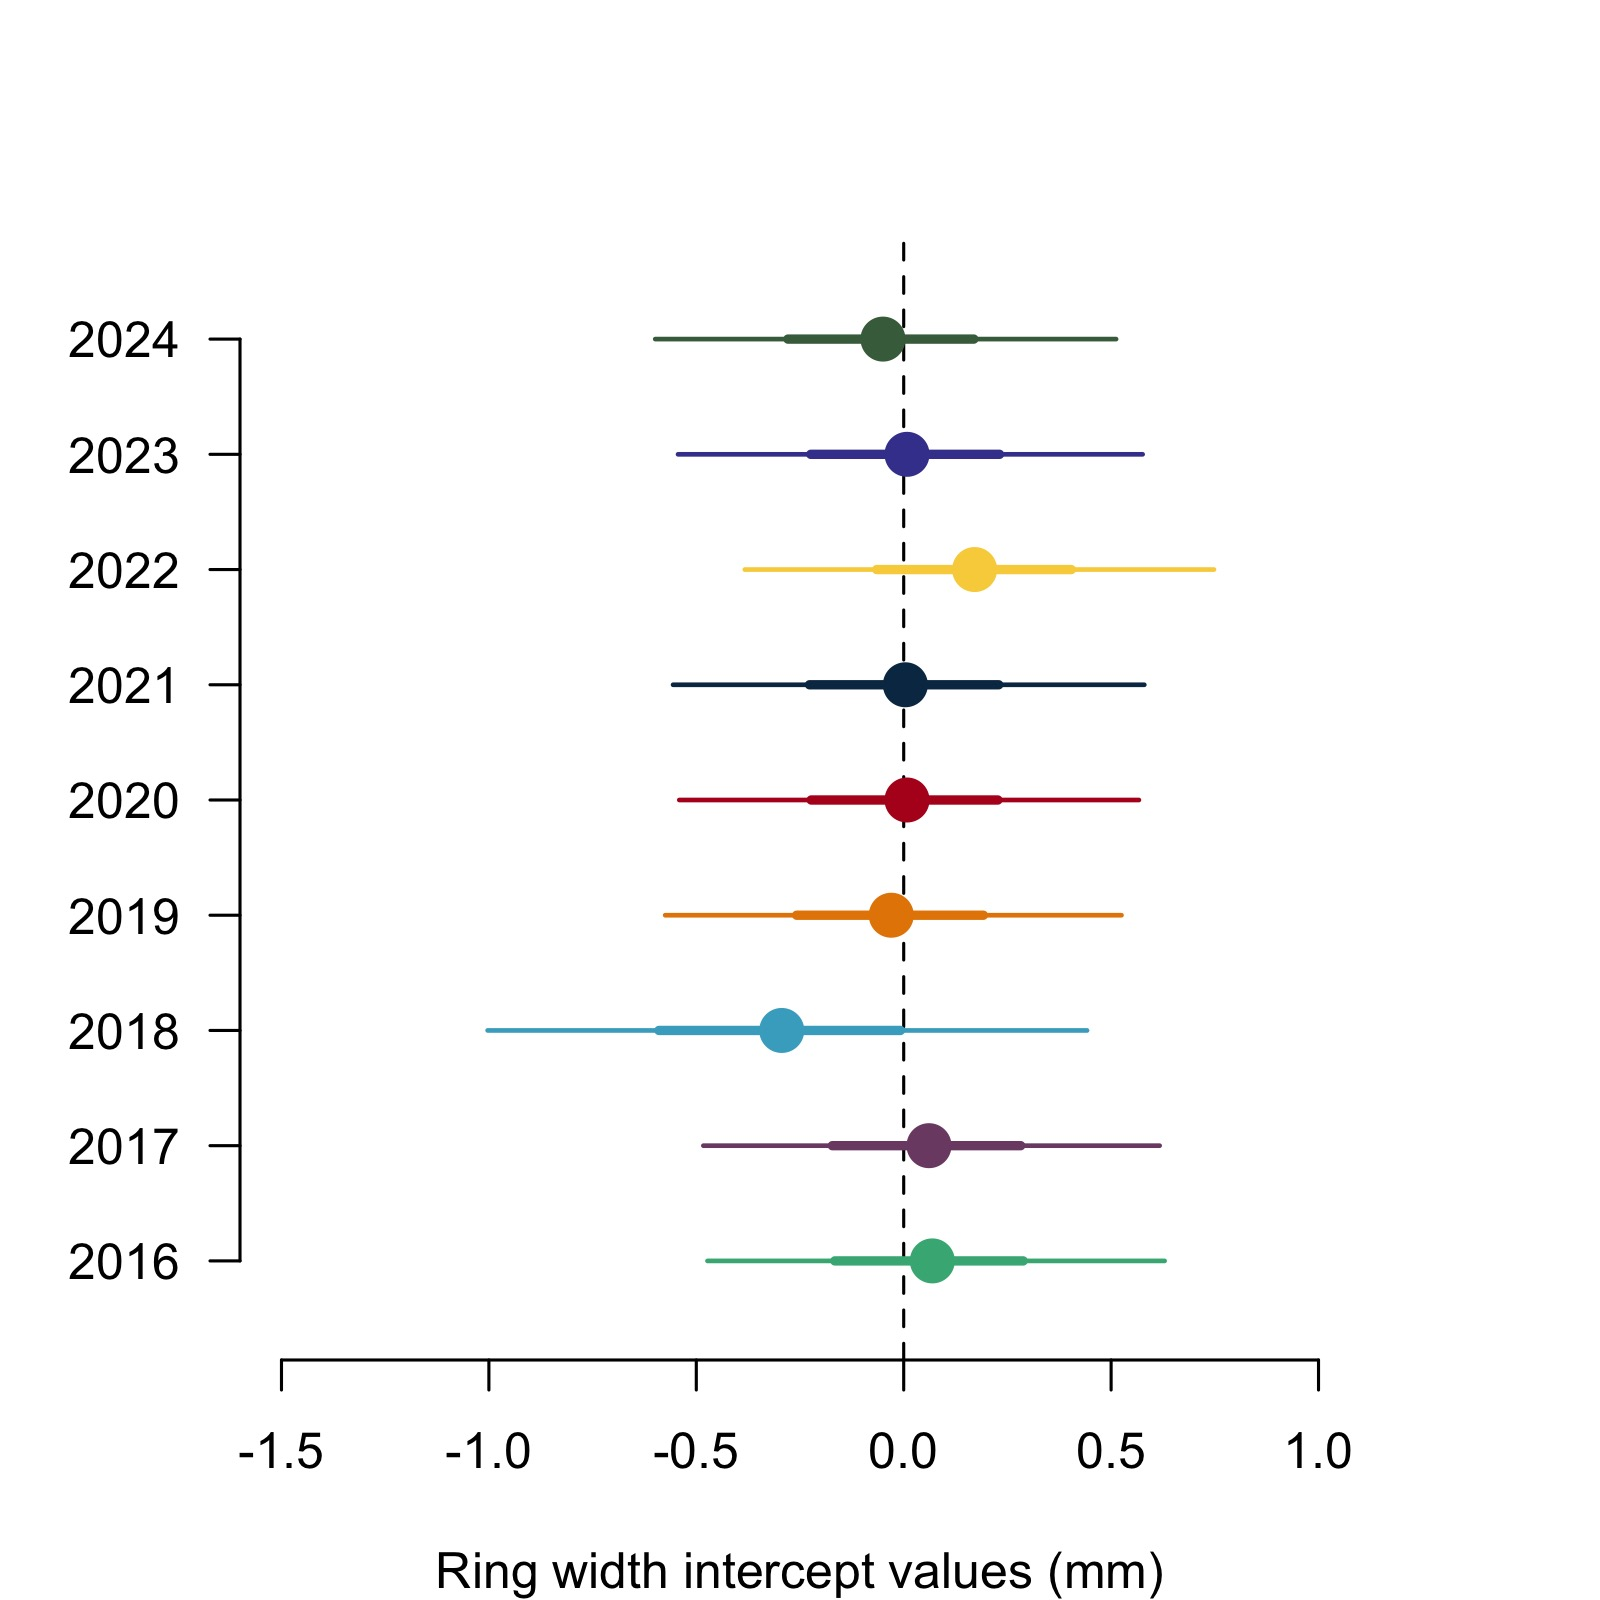
\includegraphics[width=0.5\textwidth]{../../analyses/figures/growthModelsMain/TSmuayear.jpeg}
\caption{Ring width (on the log scale) deviations from the grand mean for each year using the GDD model (Table \ref{tab:tab_all}). The dots are the mean of the posterior distribution and the thick and thin lines, the 50 and 90\% UI.}
\label{fig:tsmuplotayear}
\end{figure}

% Coringtreespotters boxplot
\begin{figure}[!ht]
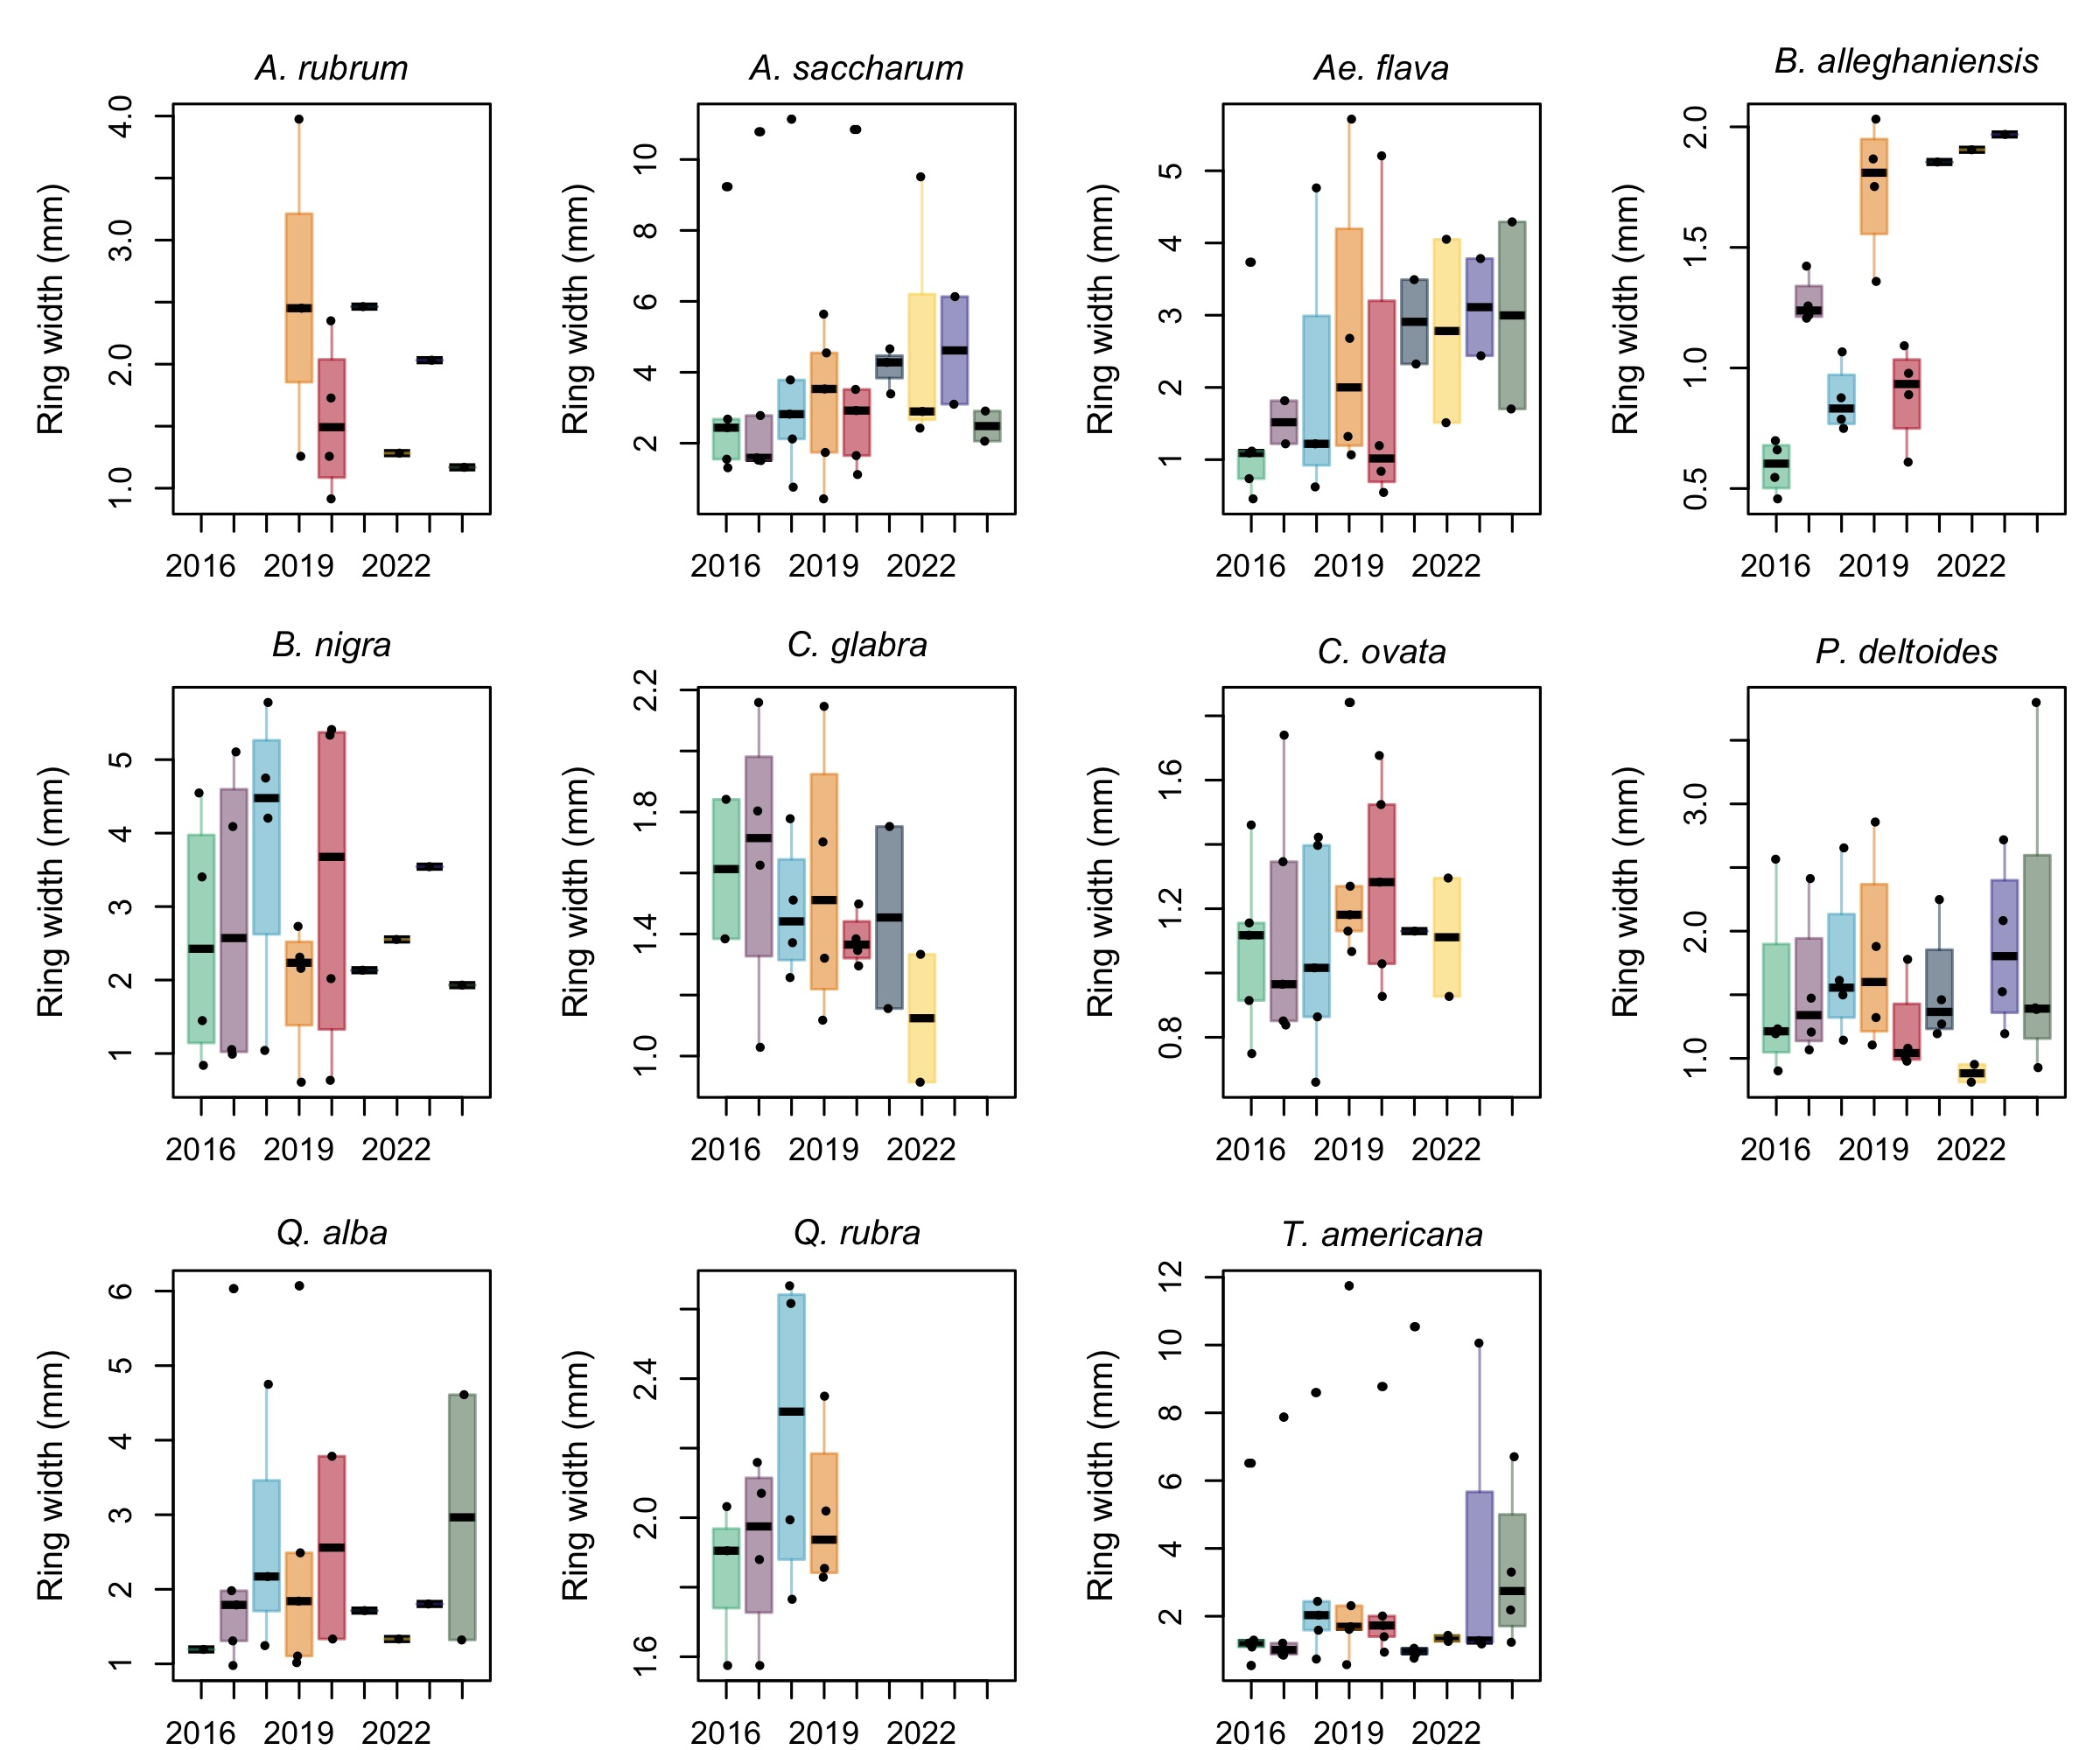
\includegraphics[width=1\textwidth]{../../analyses/figures/growthModelsMain/boxplotRingWidth.jpeg}
\caption{Boxplot representing the empirical data of our ring widths (mm) across years, facetted by species. The dots represent the raw data, the line the mean and the box the interquantile range (IQR).}
\label{fig:tsboxplot}
\end{figure}

% XY facetted by species GDD shaped by tree id
\begin{figure}[!ht]
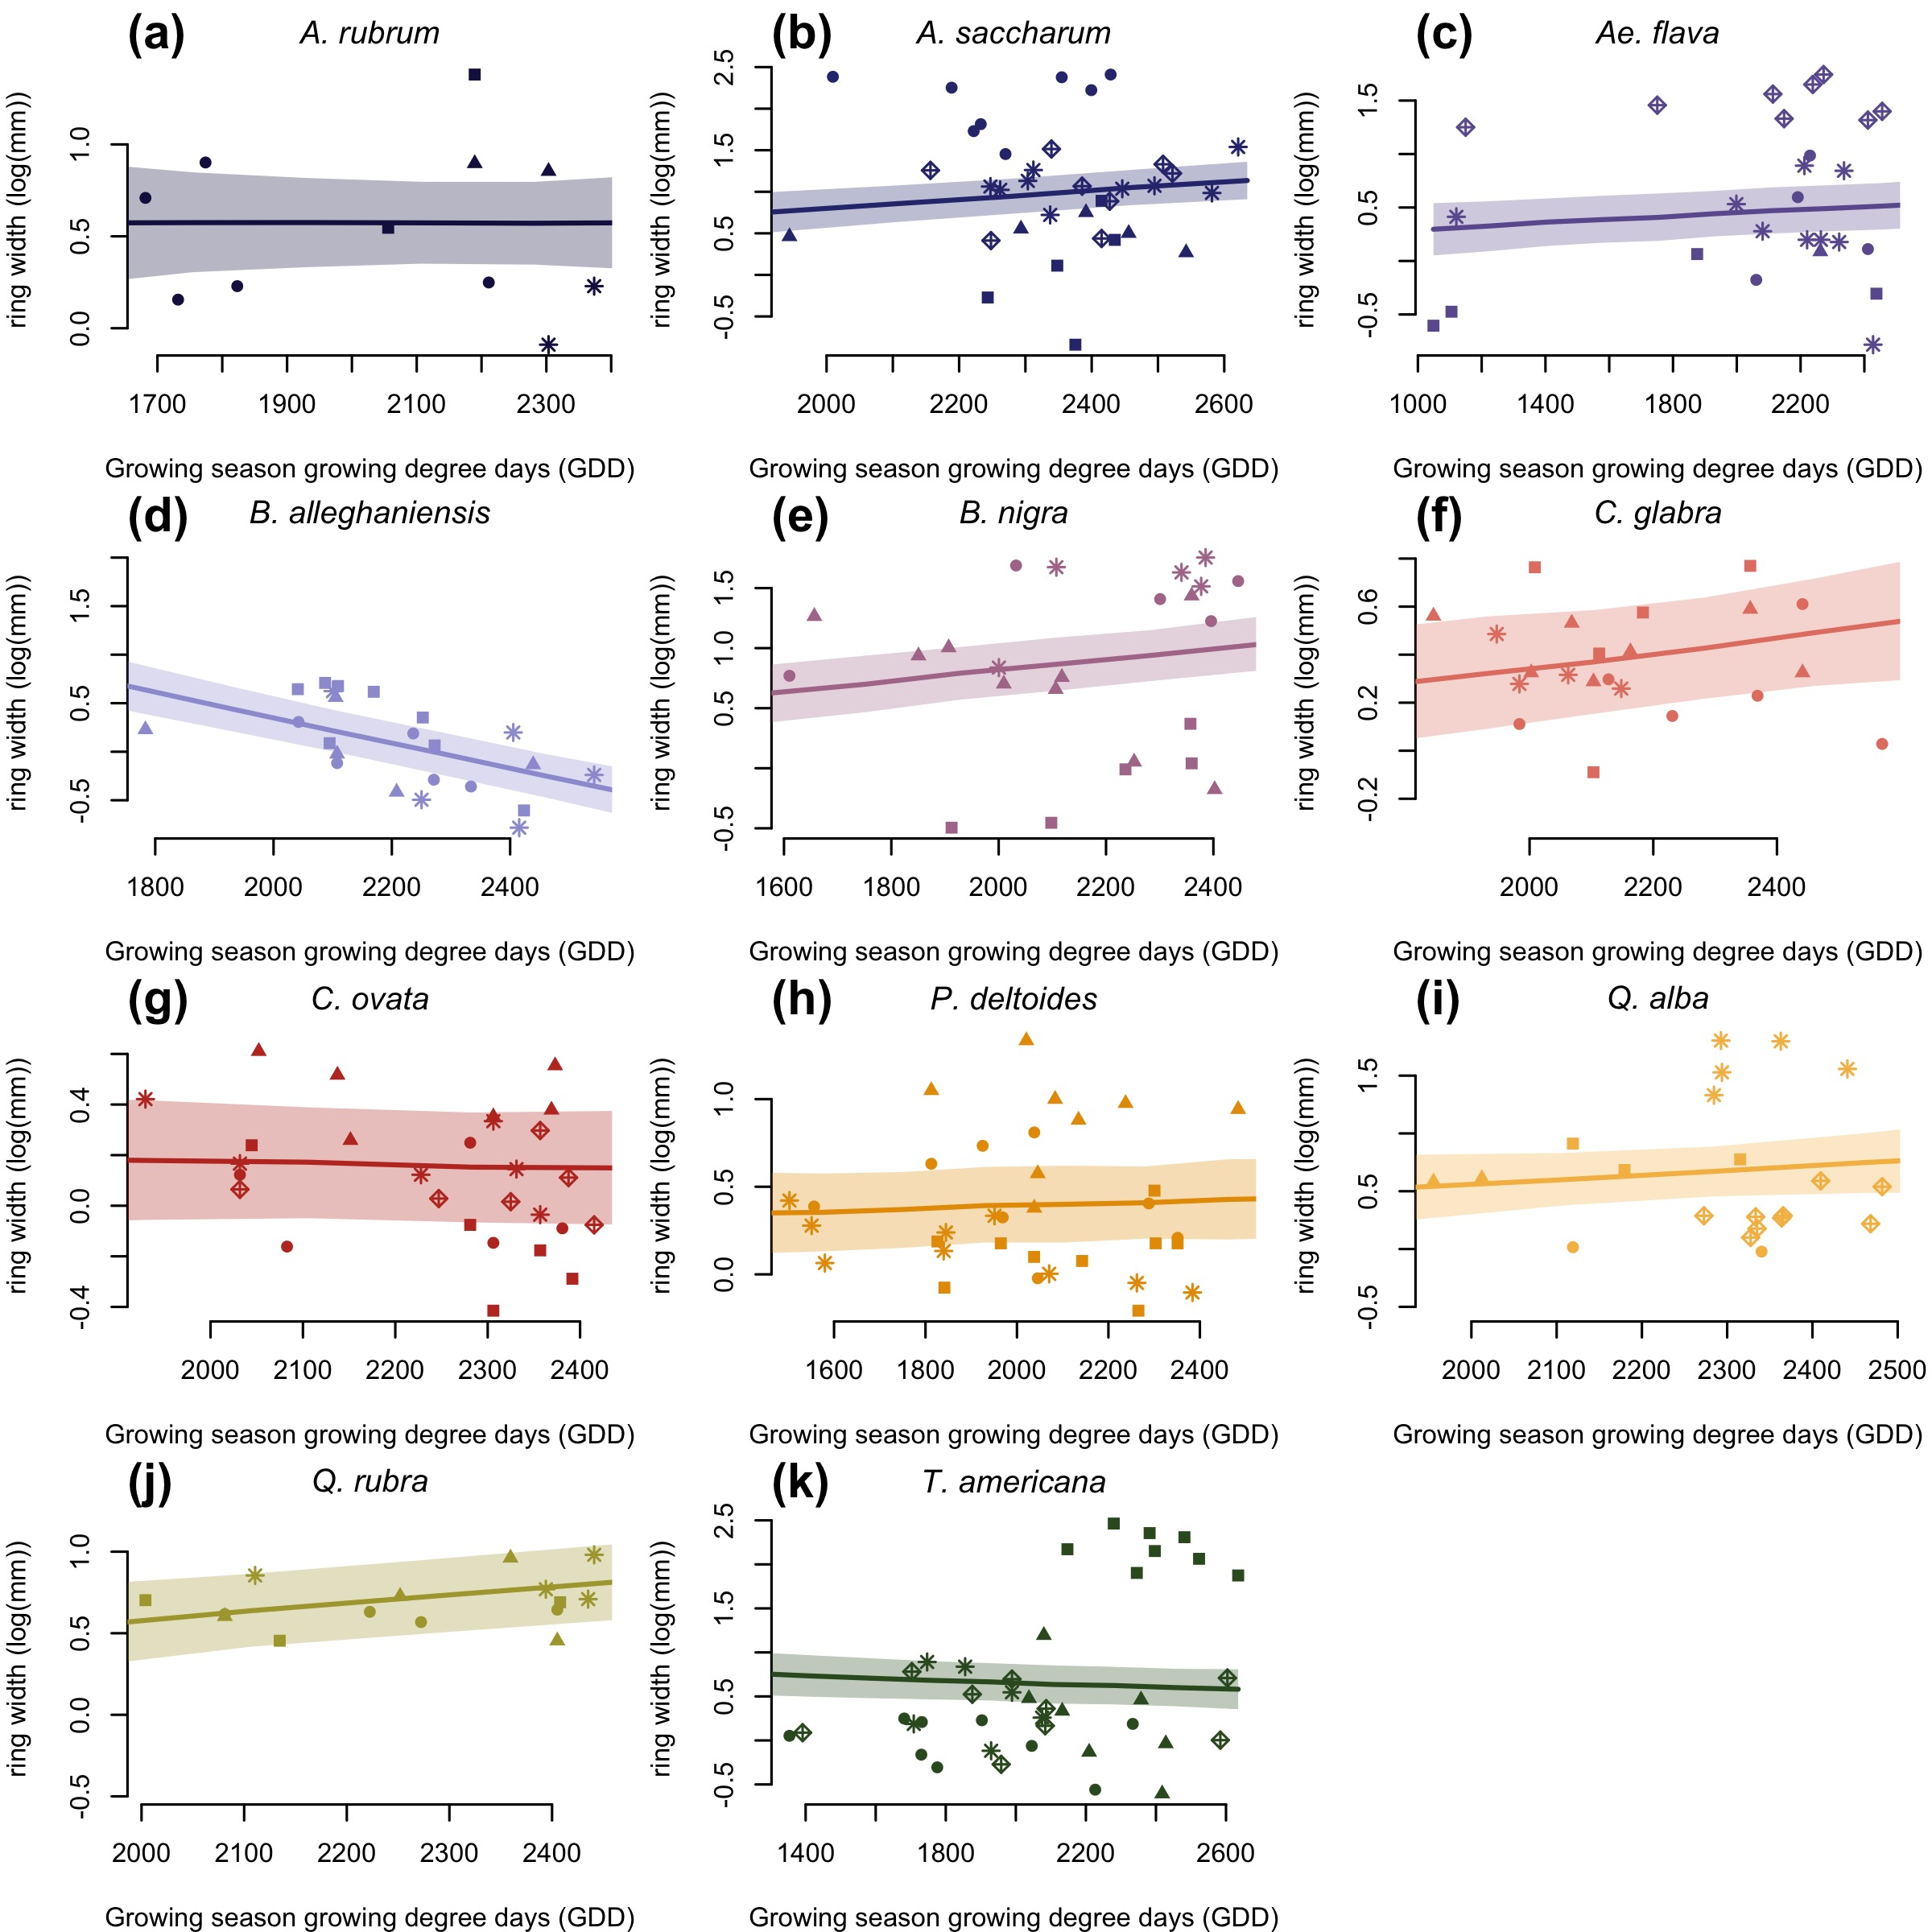
\includegraphics[width=0.8\textwidth]{../../analyses/figures/growthModelsMain/TSgrowthModelSlopesperSppFacetGDDtree.jpeg}
\caption{Ring width (on the log scale) trends in response to thermal season (GDD). The plots are the reconstructed species estimates posterior distribution with error. The lines represent the mean of the posterior distribution and the shaded area, the 50\% UI. The dots are the empirical data shaped by treeids.}
\label{fig:tsxyGDDtree}
\end{figure}

% XY facetted by species GSL shaped by tree id
\begin{figure}[!ht]
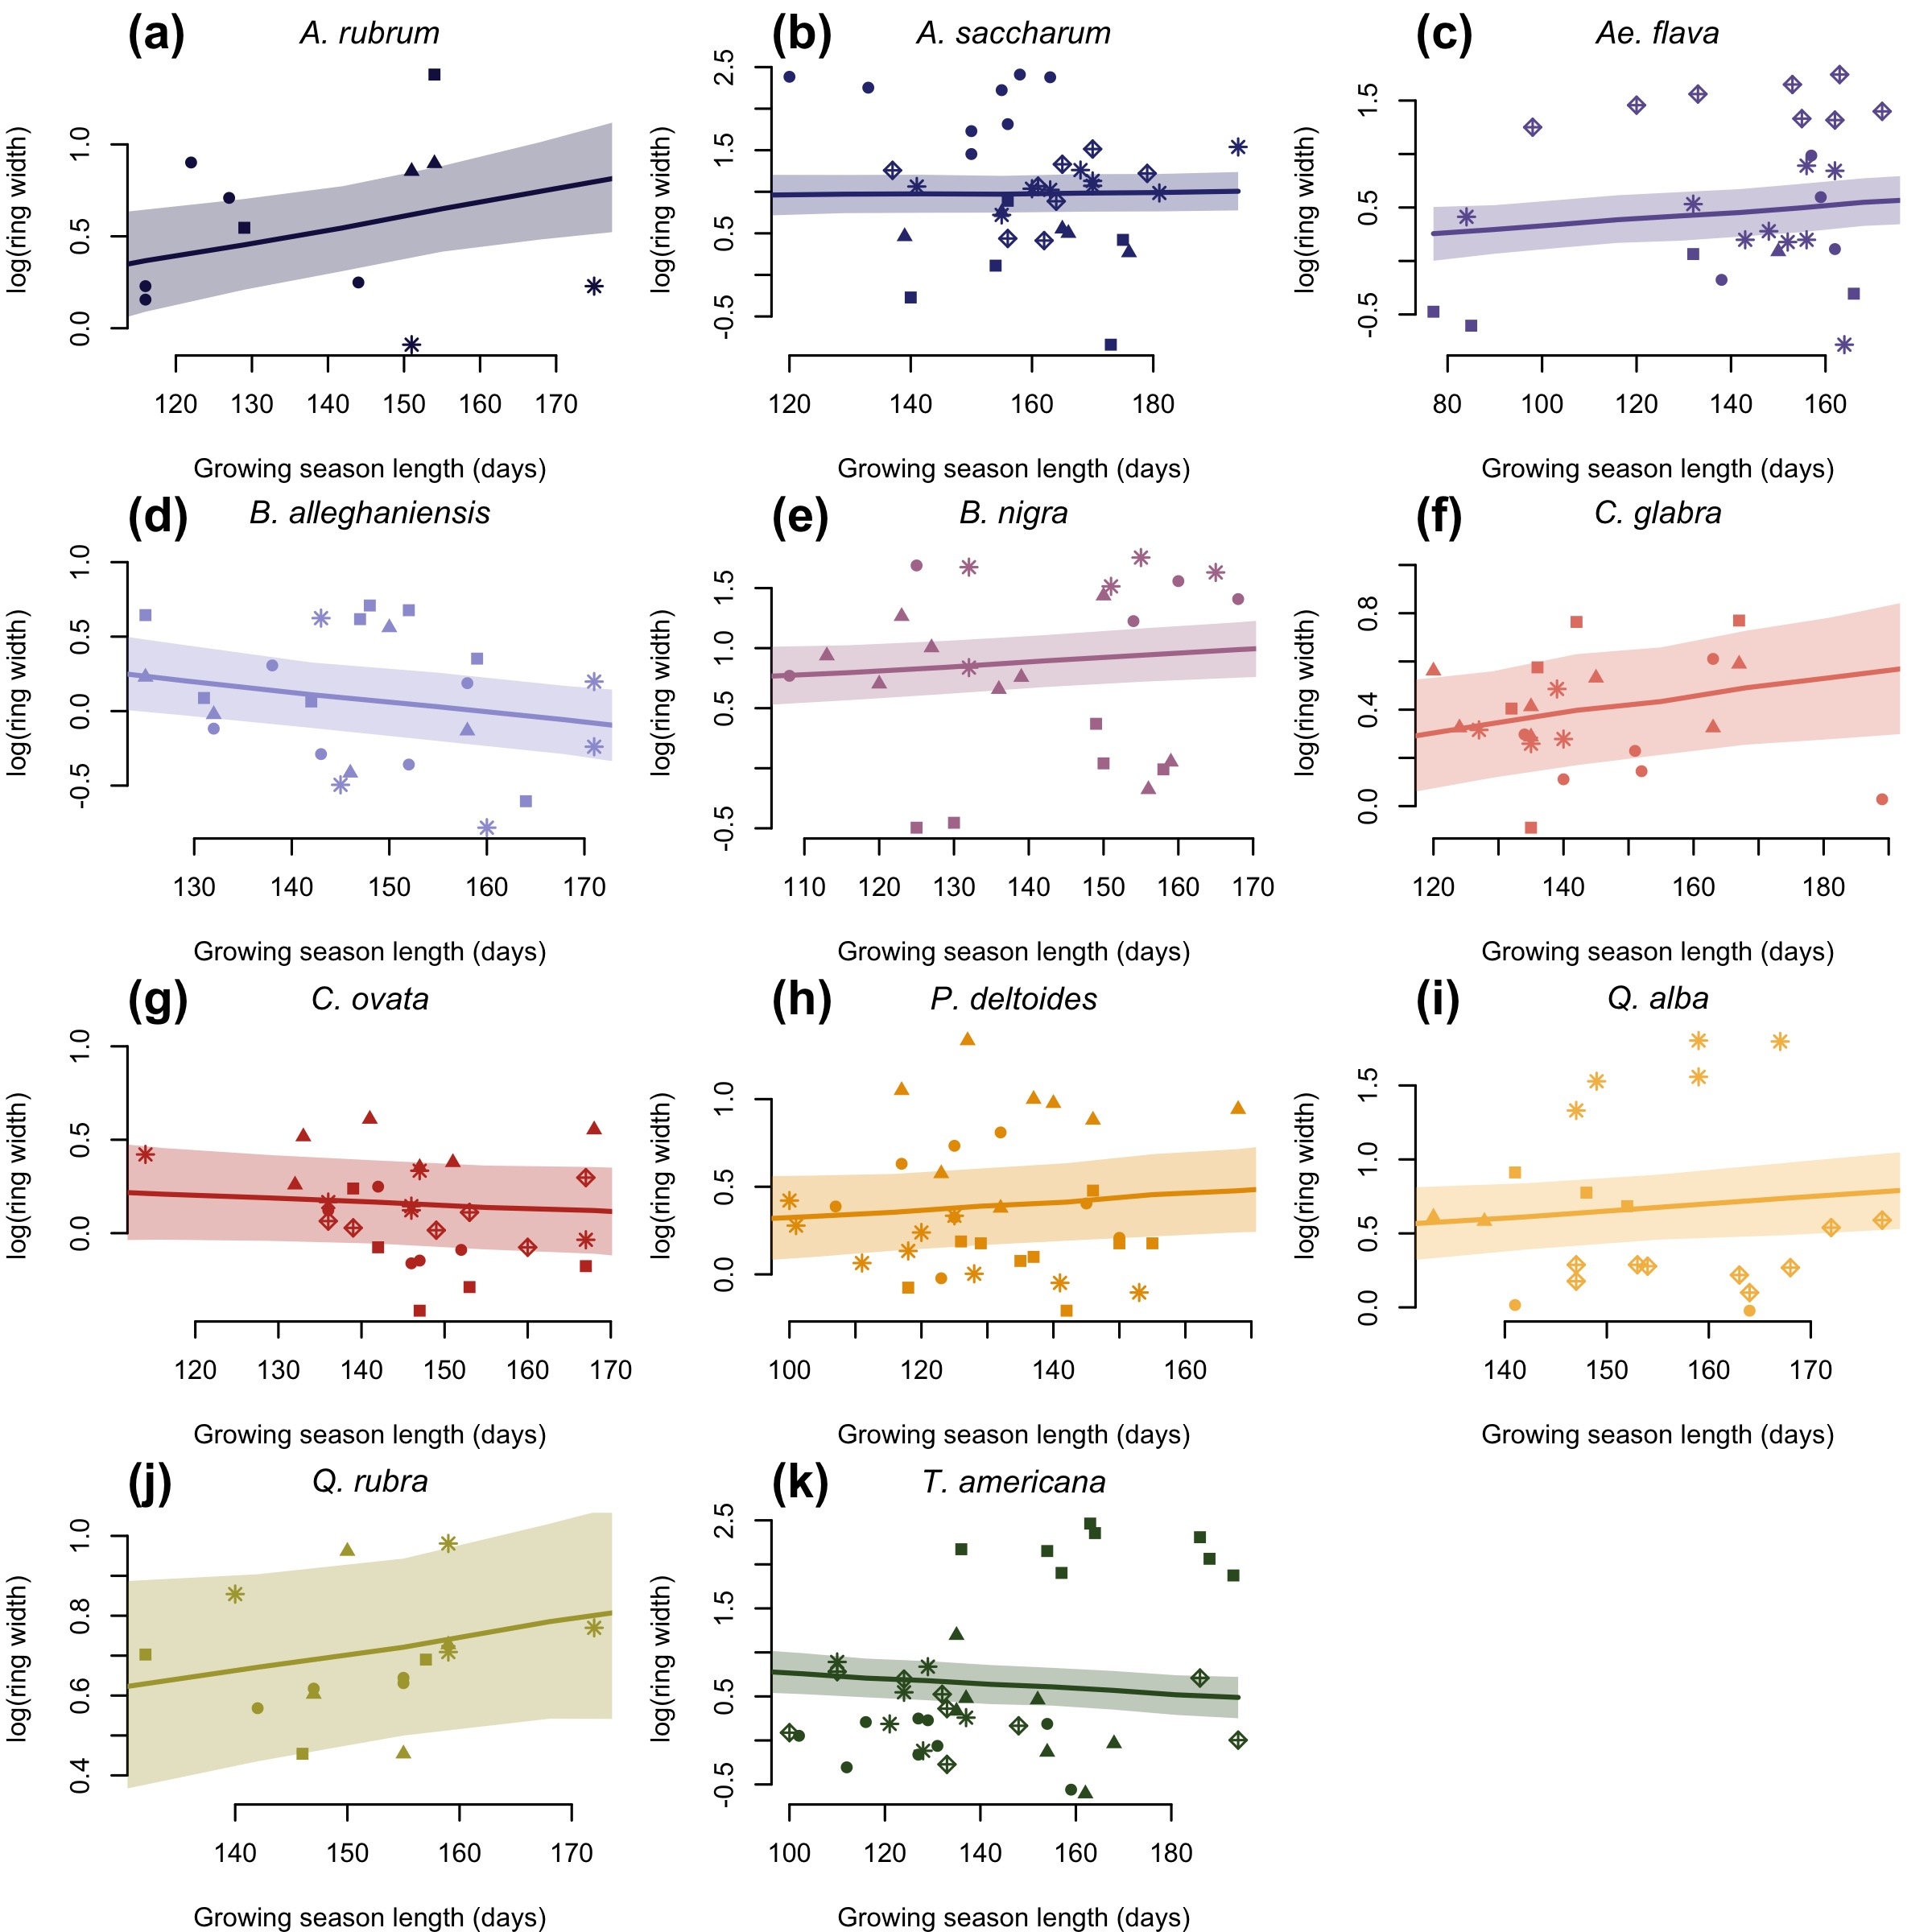
\includegraphics[width=0.8\textwidth]{../../analyses/figures/growthModelsMain/TSgrowthModelSlopesperSppFacetGSLtree.jpeg}
\caption{Ring width trends (on the log scale) in response to calendar season (GSL). The plots are the reconstructed species estimates posterior distribution with error. The lines represent the mean of the posterior distribution and the shaded area, the 50\% UI. The dots are the empirical data shaped by treeids.}
\label{fig:tsxyGSLtree}
\end{figure}

% XY facetted by species GDD shaped by year
\begin{figure}[!ht]
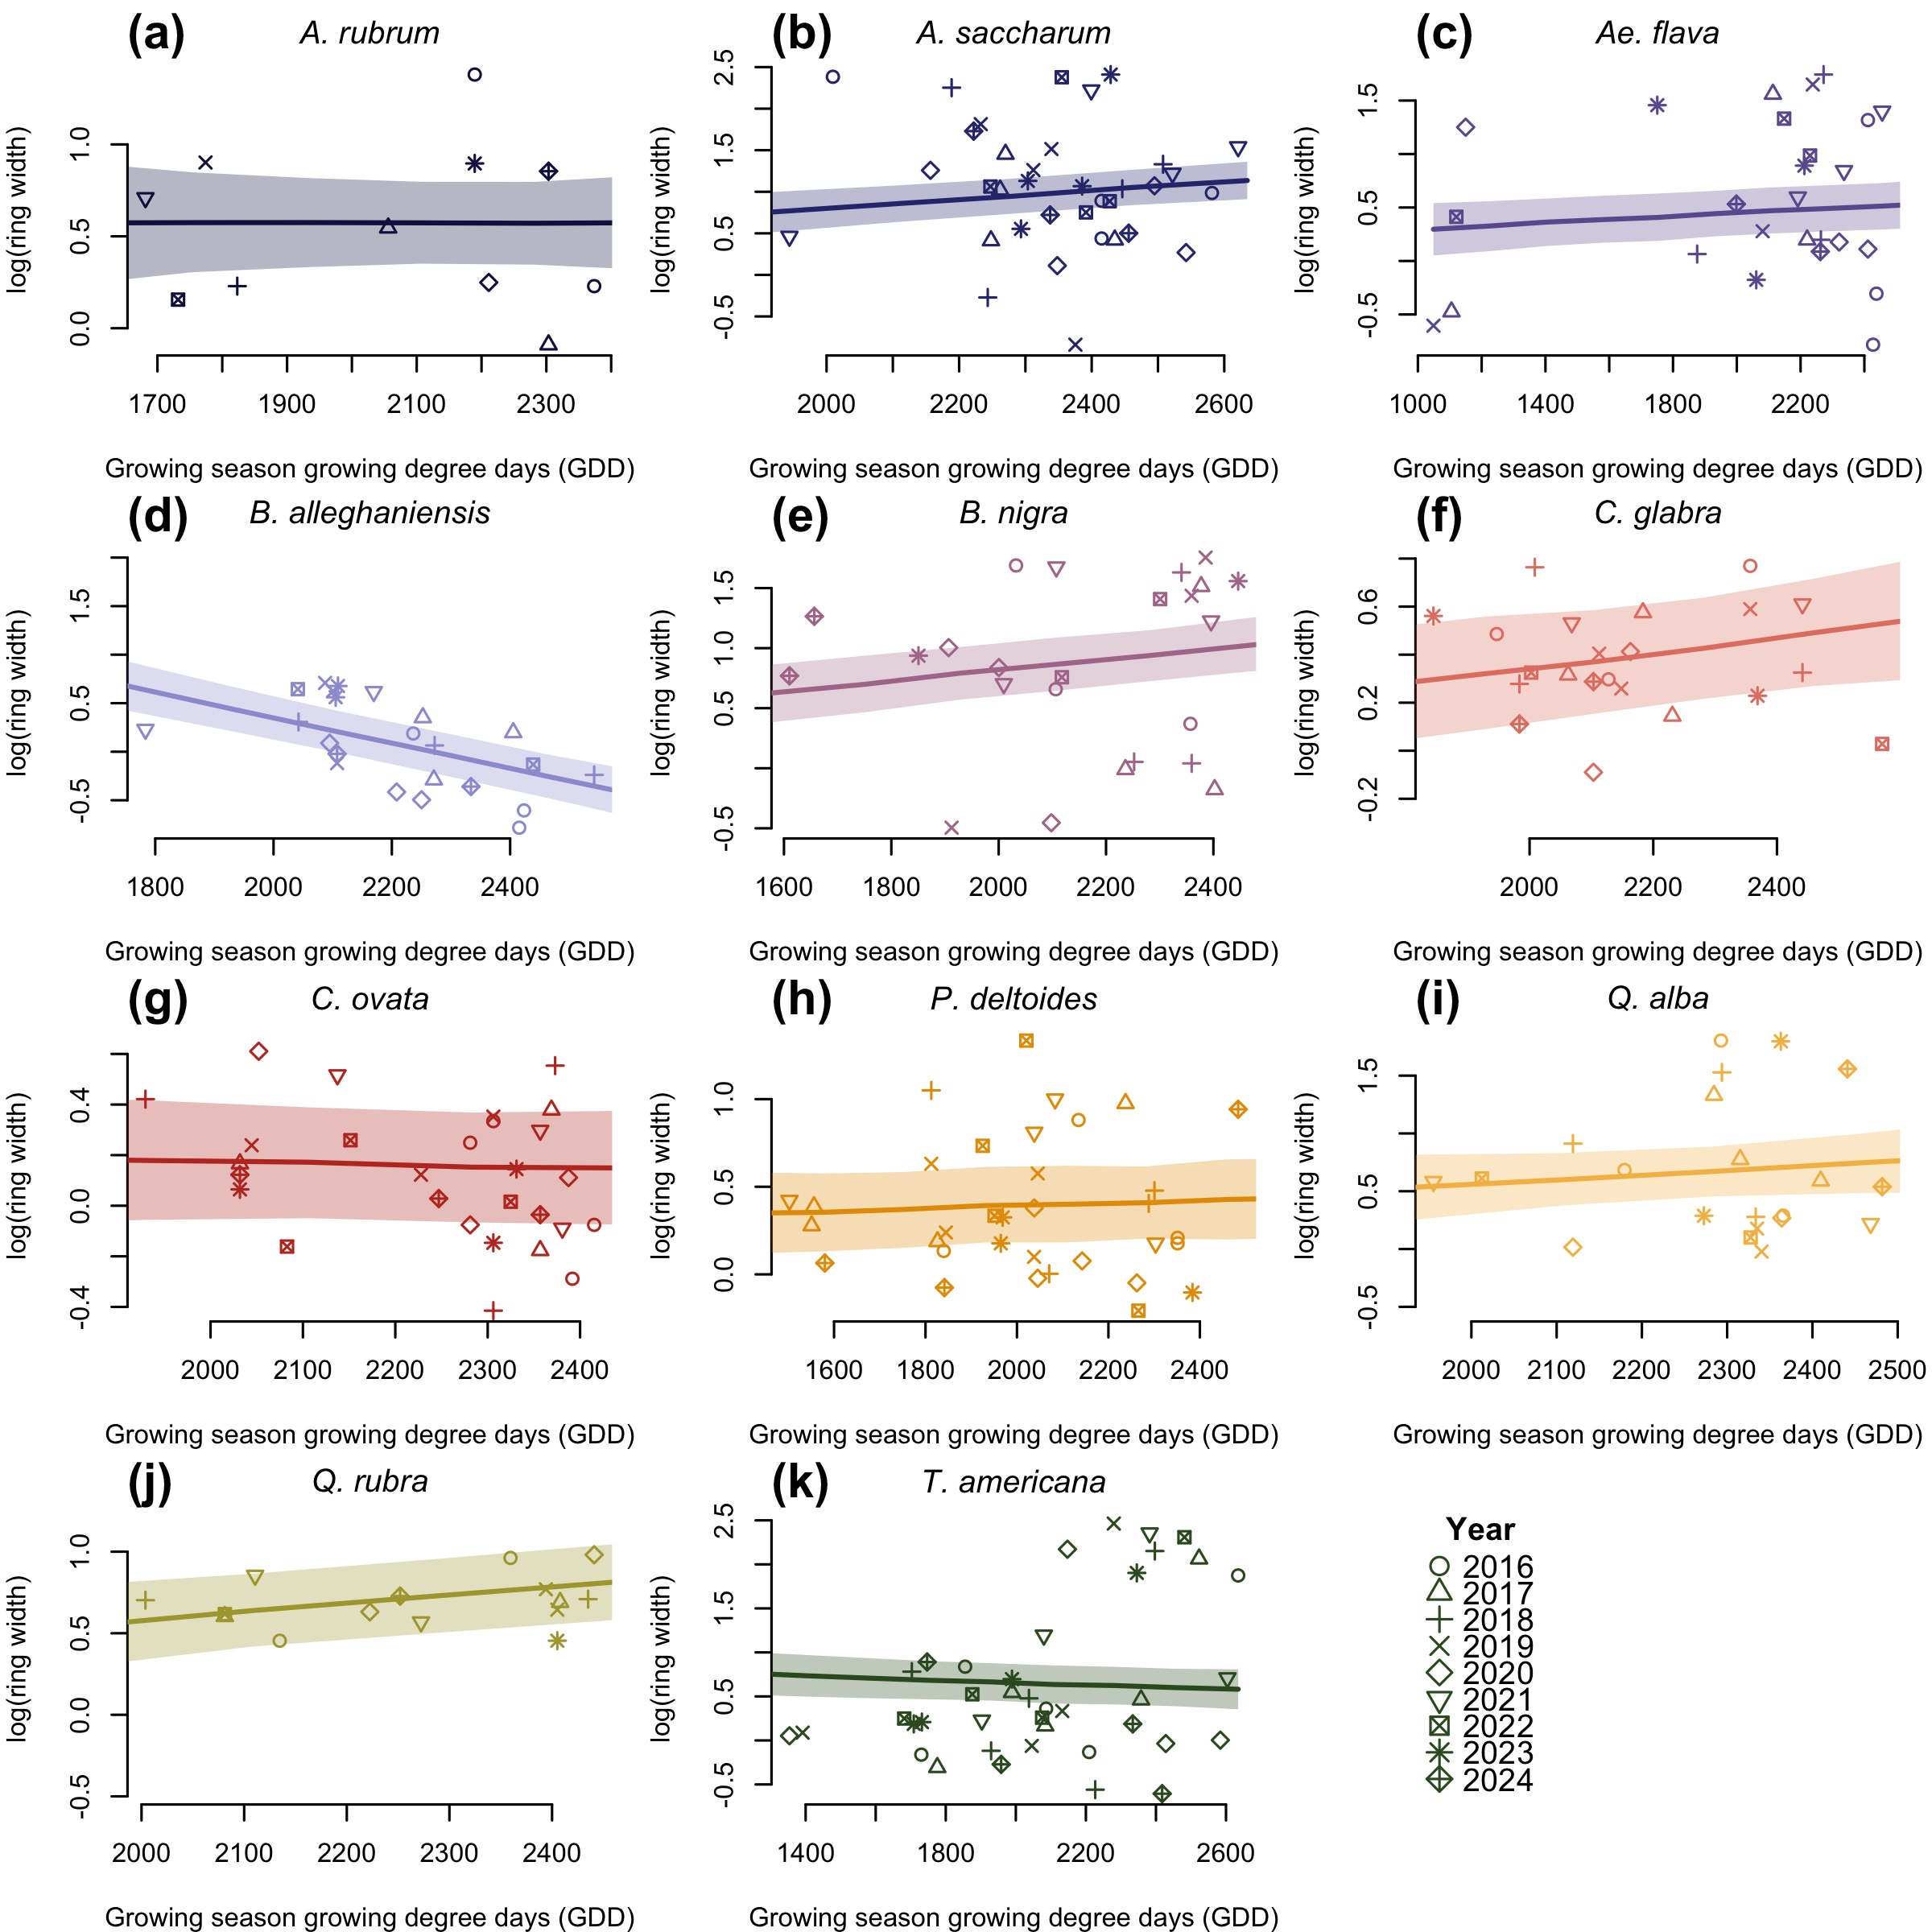
\includegraphics[width=0.8\textwidth]{../../analyses/figures/growthModelsMain/TSgrowthModelSlopesperSppFacetGDDyr.jpeg}
\caption{Ring width trends (on the log scale) in response to thermal season (GDD). The plots are the reconstructed species estimates posterior distribution with error. The lines represent the mean of the posterior distribution and the shaded area, the 50\% UI. The dots are the empirical data shaped by year.}
\label{fig:tsxyGDDyr}
\end{figure}

% XY facetted by species GSL shaped by year
\begin{figure}[!ht]
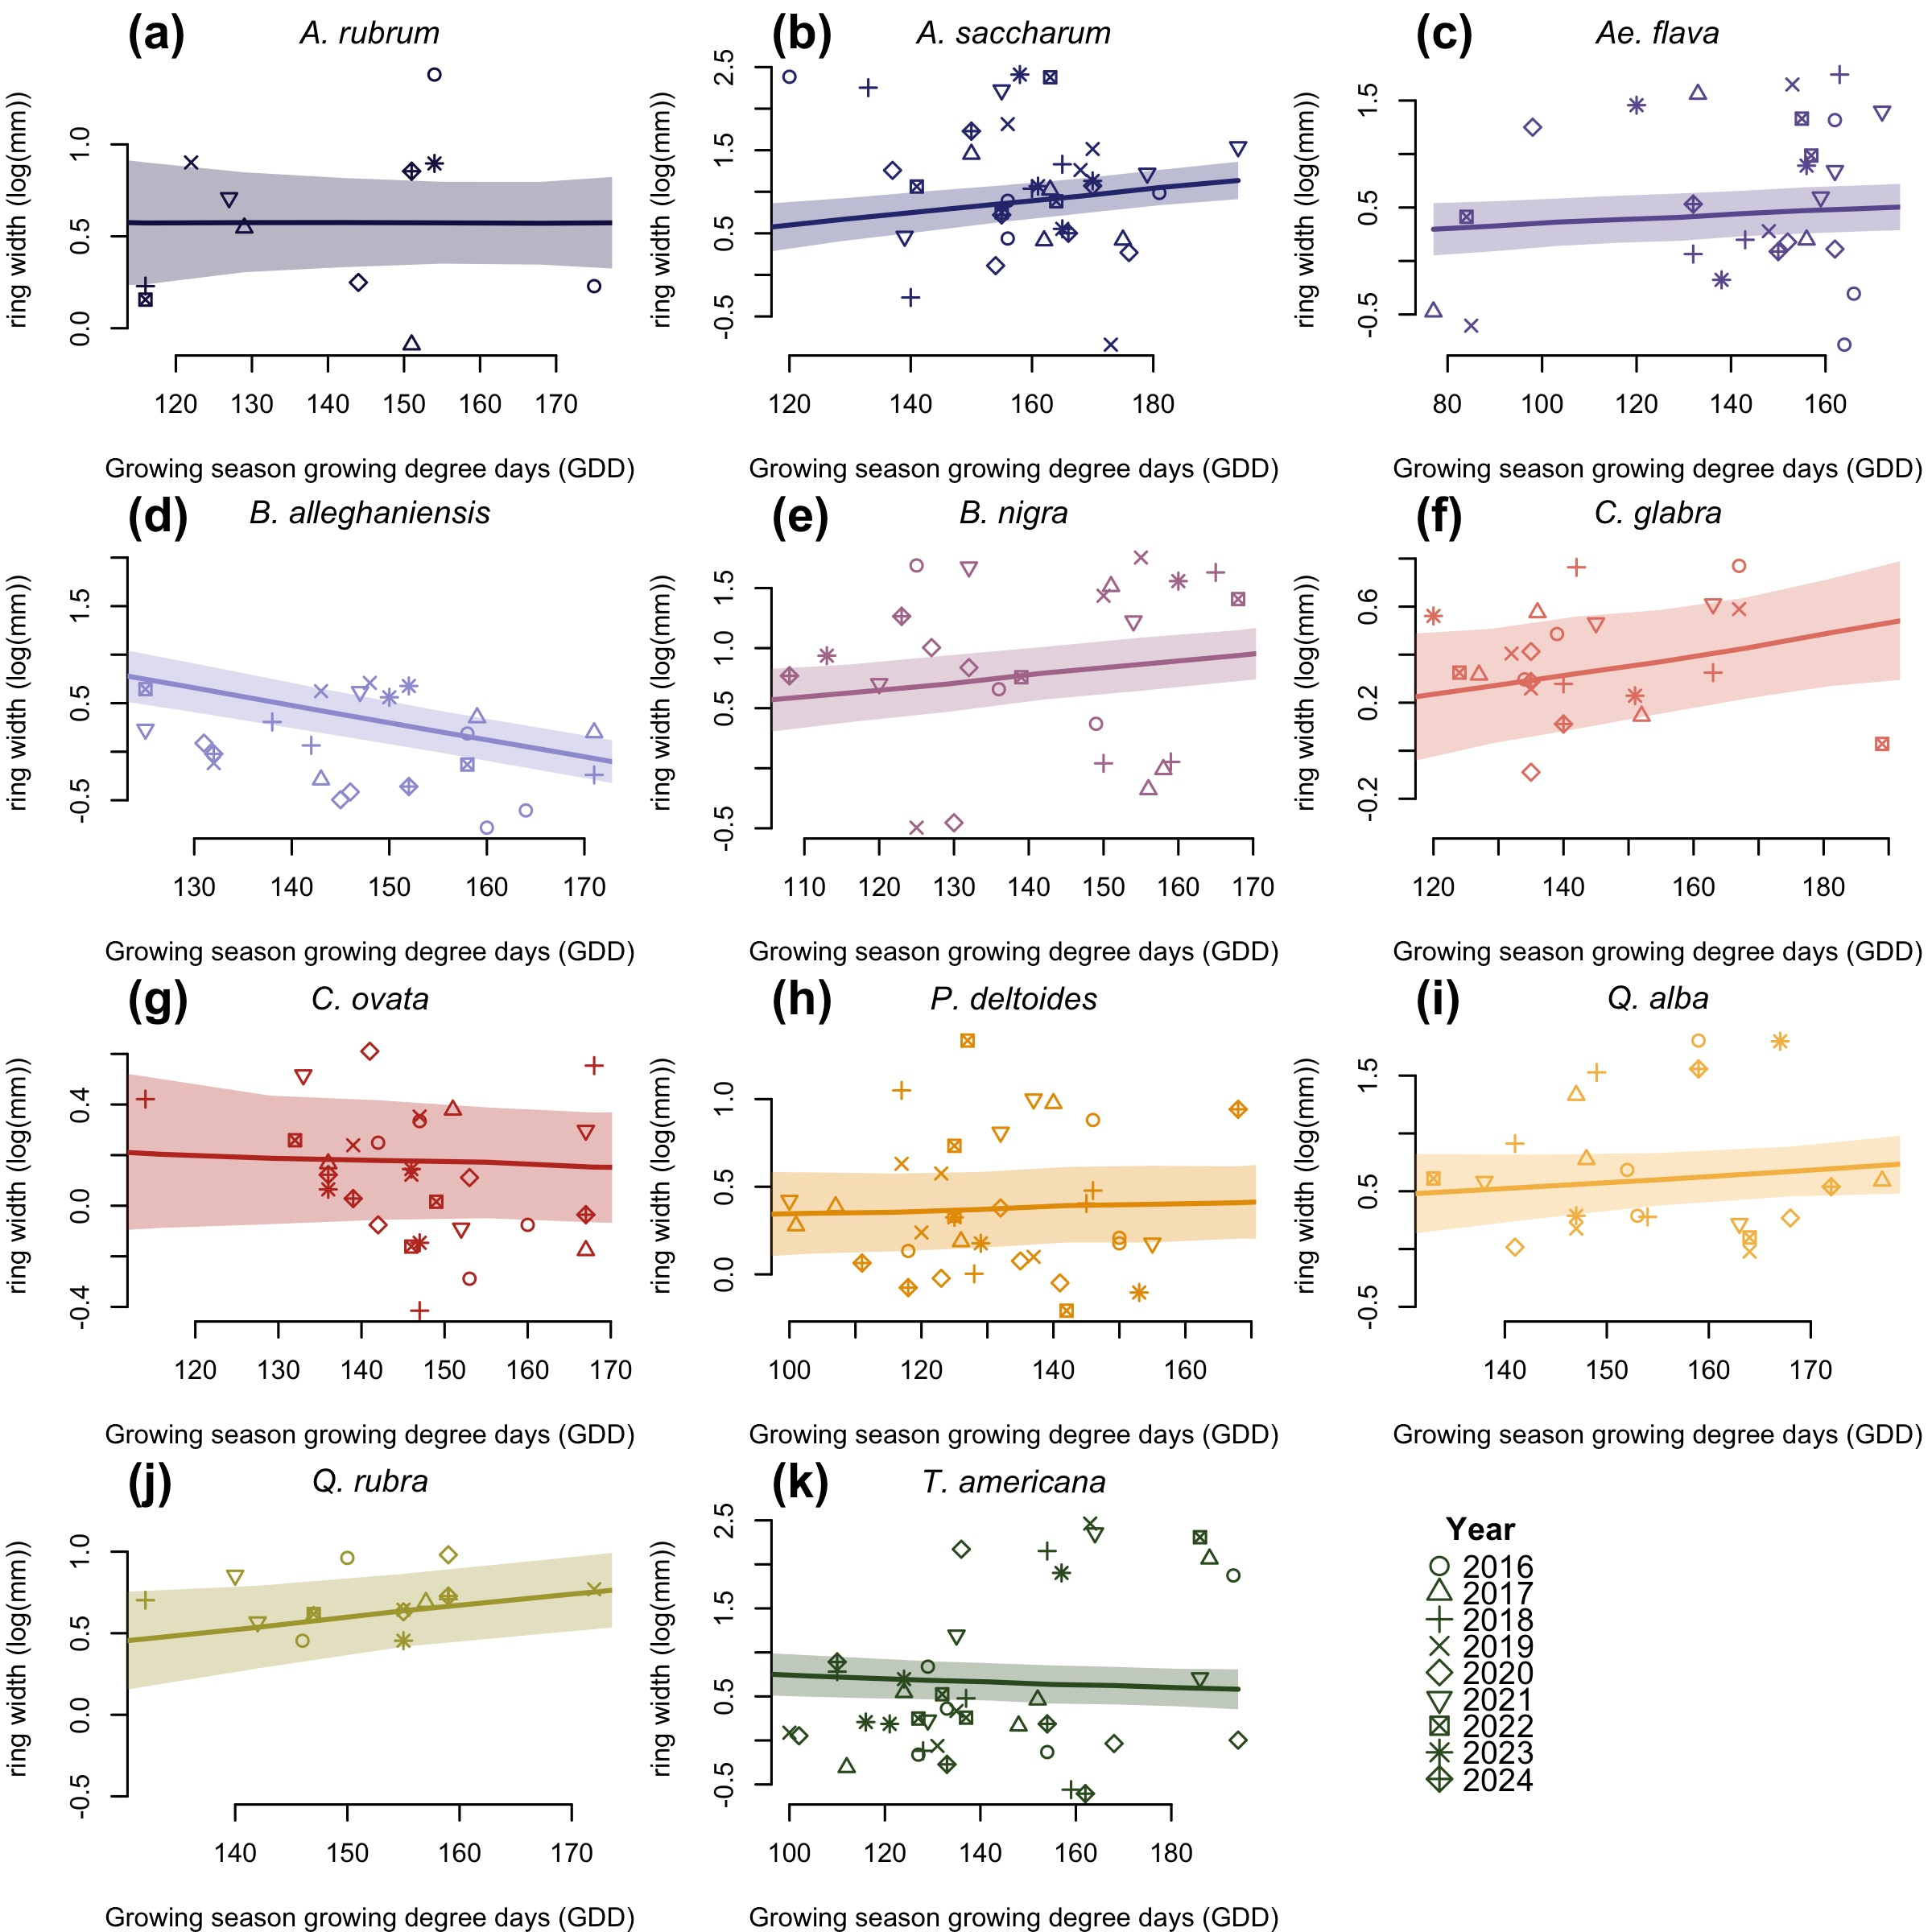
\includegraphics[width=0.8\textwidth]{../../analyses/figures/growthModelsMain/TSgrowthModelSlopesperSppFacetGSLyr.jpeg}
\caption{Ring width trends (on the log scale) in response to calendar season (GSL). The plots are the reconstructed species estimates posterior distribution with error. The lines represent the mean of the posterior distribution and the shaded area, the 50\% UI. The dots are the empirical data shaped by year.}
\label{fig:tsxyGSLyr}
\end{figure}

% Figure mu atreeid full
\begin{figure}[!ht]
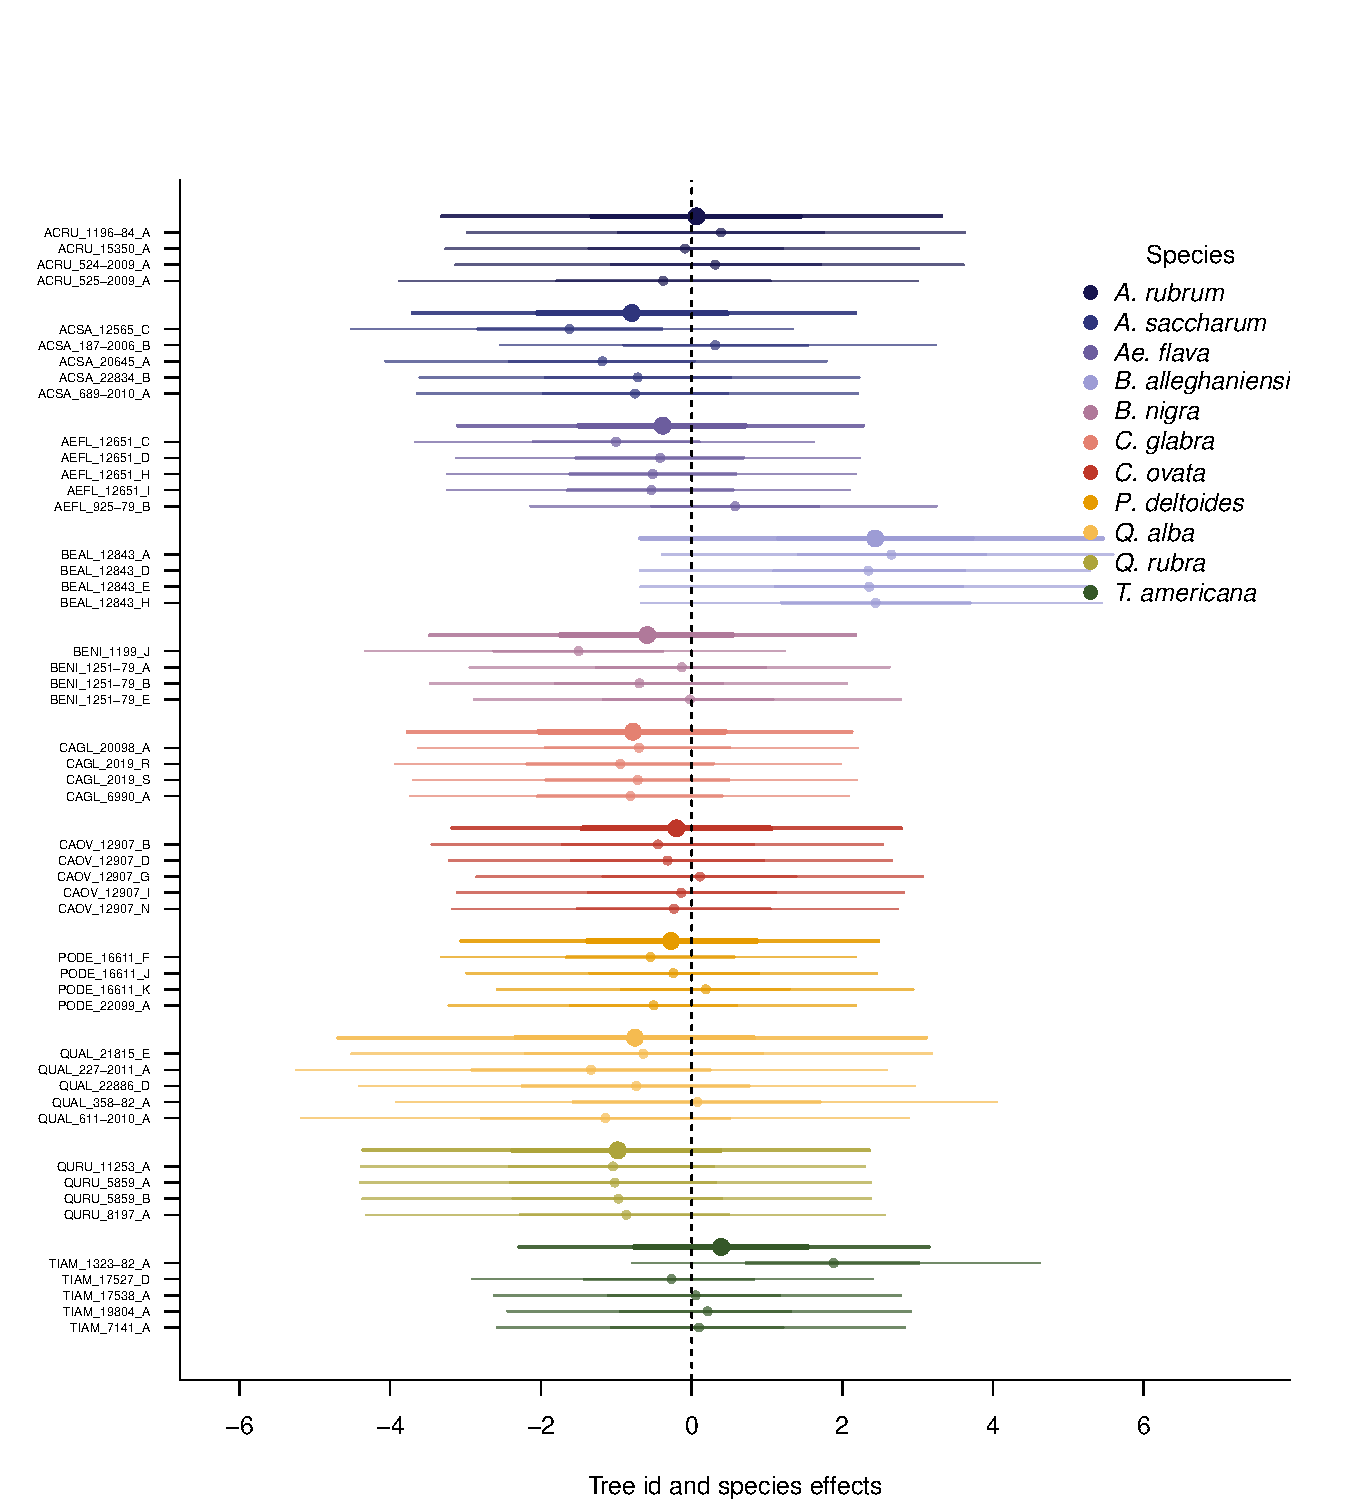
\includegraphics[width=0.8\textwidth]{../../analyses/figures/growthModelsMain/TSmeanPlotGrowthGDD_treeidBYspp.pdf}
\caption{Ring width (on the log scale) deviations from the grand mean for each grouping factor of the GDD model. The different tree id values represent the combined intercepts of tree id, species and averaged year intercepts. The larger dots and lines represent the species intercepts which are the species level estimates averaged across all of their tree ids. The dots are the mean of the posterior distribution and the thick and thin lines, the 50 and 90\% UI.}
\label{fig:tsmuplotatreeid}
\end{figure}

% Full vs restricted data comparison for Coringtreespotters
\begin{figure}[!ht]

\includegraphics[width=1\textwidth]{/Users/christophe_rouleau-desrochers/github/coringtreespotters/analyses/figures/growthModelsMain/FullVSRestricted.pdf}
\caption{Full vs most restricted rows of data for the model with SOS (a) EOS (b) as the predictor. Each pannel represent the different parameters used to fit the models (see data analyses for more details).}
\label{fig:tsSOSEOScomparison}
\end{figure}

% Budburst vs leafout for CoringTreespotters
\begin{figure}[!ht]

\includegraphics[width=0.8\textwidth]{/Users/christophe_rouleau-desrochers/github/coringtreespotters/analyses/figures/growthModelsMain/budburstVSLeafout/DporousVSRporous.jpeg}
\caption{Parameter estimates when calculating the GDD (a), GSL (b) from leafout vs budburst, to leaf coloring. (c) shows the model estimates when taking leafout vs budburst as the SOS (see data analyses for more details).}
\label{fig:buburstVSleafoutTS}
\end{figure}

% Z-scored slope results
\begin{figure}[!ht]
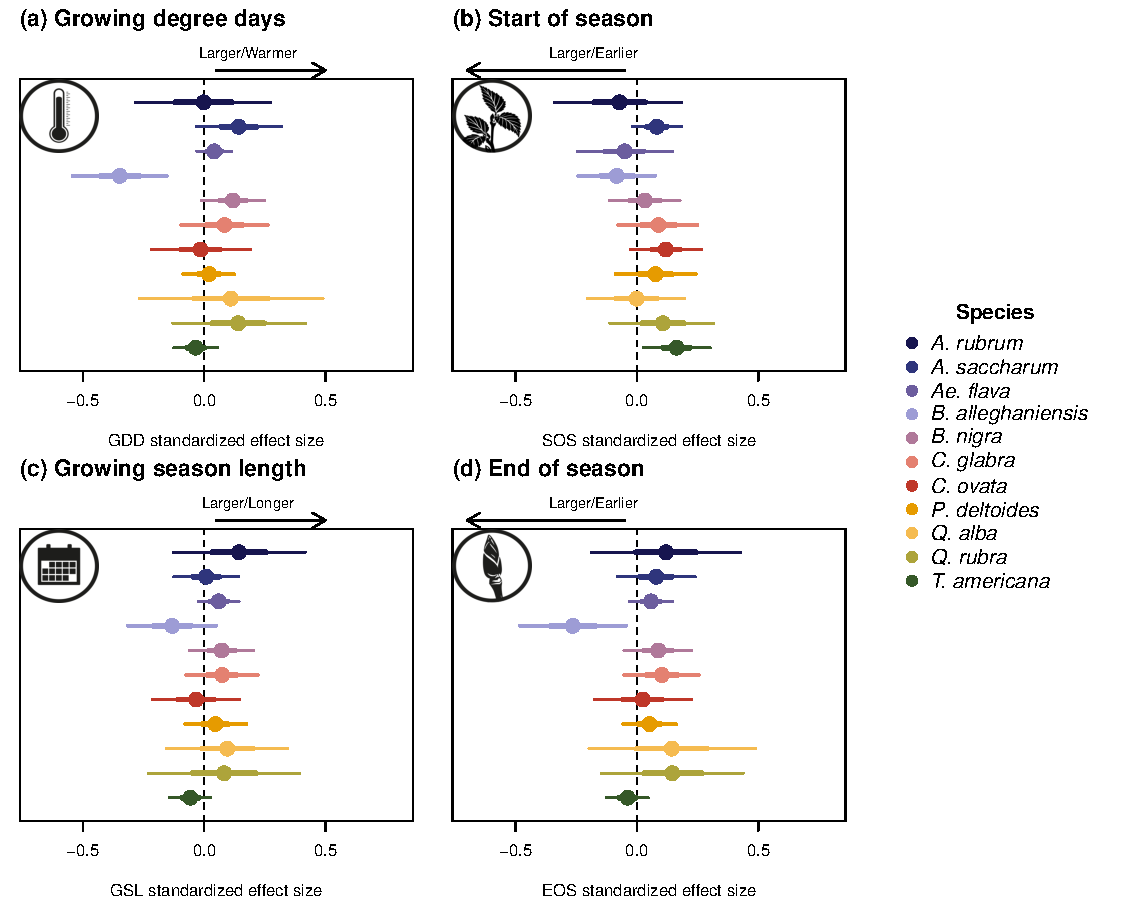
\includegraphics[width=0.8\textwidth]{../../analyses/figures/growthModelsMain/zscored/muALLbsppZ.pdf}
\caption{Effect size of each predictors across our eleven species. We depict ring width (on the log scale) change per scaled (z-scored; see data analyses section for more details) predictor for each species. We report estimates as mean and 90\% uncertainty intervals (in square brackets) across our four different predictors (GDD: growing degree days, GSL: growing season length, SOS: start of season and EOS: end of season).}
\label{fig:bsppZscored}
\end{figure}

% Carry over of SOS on EOS
\begin{figure}[!ht]
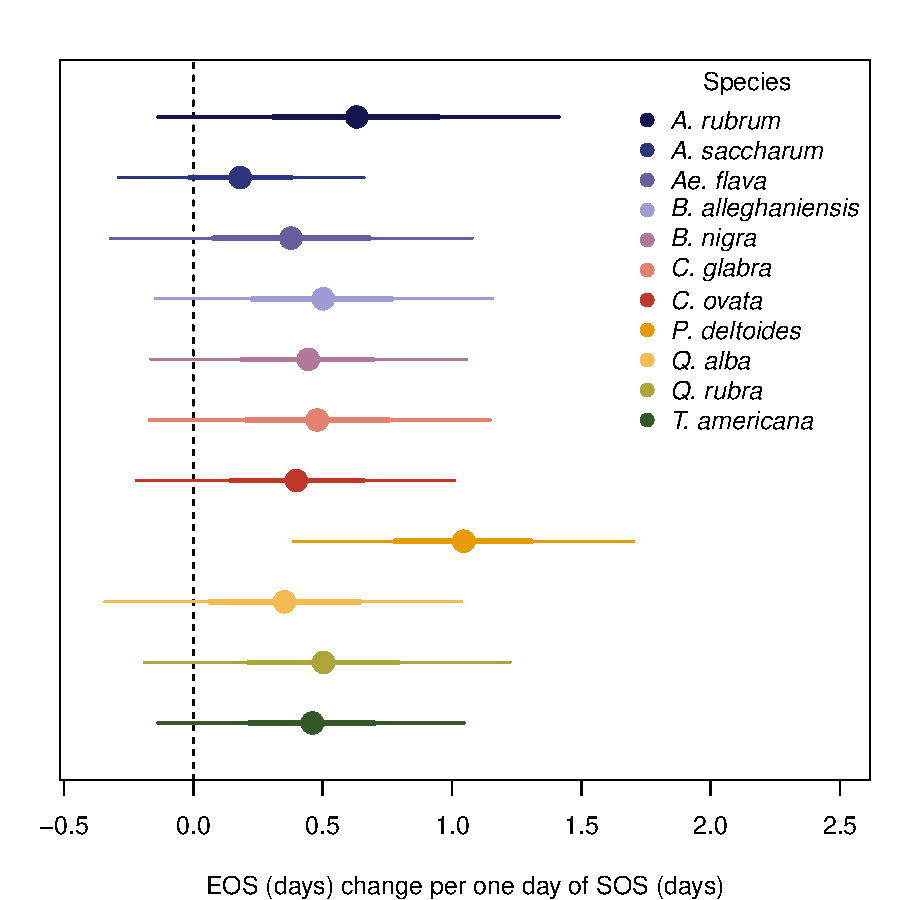
\includegraphics[width=0.8\textwidth]{../../analyses/figures/SOSonEOS/bsppSOSonEOS.pdf}
\caption{Effect of the start of season (SOS) on the end of season (EOS) across our eleven species. We report these slope estimates as mean and 90\% uncertainty intervals.}
\label{fig:SOSonEOS}
\end{figure}

%<><><><><><><><><><><><><><><><><><><><><><><><><><><><><><><><><><><><><><><><>
% REFERENCES %
%<><><><><><><><><><><><><><><><><><><><><><><><><><><><><><><><><><><><><><><><>
\clearpage
\bibliography{ExportedItems}
\bibliographystyle{besjournals} 

\end{document}
